\stopallthesefloats
\subsection{Evaluating Interference Through Resource-Stressing}
\label{sec:radojkovic}
\cite{10.1145/2086696.2086713} presents a strategy to characterize the
sensibility of a shared resource to temporal interference. The general idea
behind the approach is to perform a stressing benchmark on an architecture's
resource with only that single thread running (i.e.~running in isolation), and
compare the result with the same test in which multiple threads of the stressing
benchmark run in parallel, in a metric called \textit{slowdown factor} (see
Definition~\ref{def:slowdown-factor}).

\begin{definition}[Slowdown Factor]
\label{def:slowdown-factor}
Given a benchmark targeting a specific component, its application using a single
thread in isolation resulting in a execution time $n$, and its application while other
threads are stressing components (potentially the same one) yielding a execution time
of $m$, the slowdown factor $f$ is defined as:
\[f = \frac{n}{m}\]
\end{definition}

This slowdown factor indicates how sensible the component targeted by the
measured benchmark is to interference, and thus how large the execution time
variations caused by parallel access to that component will be. By having the
other threads target different components, correlation between them can be
exposed: if the slowdown factor is higher than $1.0$, some interactions occur
between these components, and the other components are able to generate
interference on any application using the component targeted by the measured
thread.
\begin{figure}[hbt!]
\begin{center}
%\lstinputlisting{\chapterdirectory/figure/micro_bench/atom_bench.txt}
\begin{tabular}{r|l|l}
\hline
Line  & Source code                    & Explanation\\
\hline
001   & {\lstinline!movl %1, %ecx!}    & initialize loop counter \textit{ecx}
({\lstinline!%1!} is an input parameter)\\
002   & {\lstinline!label_intAdd:!}    & beginning of the loop\\
003   & {\lstinline!add %eax, %ebx!}   & target instruction\\
004   & {\lstinline!add %ebx, %eax!}   & target instruction\\
...   & {\lstinline!...!}              & ...\\
...   & {\lstinline!...!}              & ...\\
252   & {\lstinline!add %ebx, %eax!}   & target instruction\\
253   & {\lstinline!decl %ecx!}        & decrement loop counter\\
254   & {\lstinline!cmp %ecx, $0!}     & compare loop counter with 0\\
255   & {\lstinline!jne label_intAdd!} & if (counter != 0) jump to the beginning of the loop\\
\hline
\end{tabular}
\end{center}
\caption{\textit{intAdd} Benchmarking Code (taken from
\cite{10.1145/2086696.2086713})}%
\label{fig:micro_bench:atom_bench}
\end{figure}

\begin{figure}[hbt!]
\begin{center}
\lstinputlisting{\chapterdirectory/figure/micro_bench/atom_init.txt}
\end{center}
\caption{Memory Benchmark Initialization Code (taken from
\cite{10.1145/2086696.2086713})}%
\label{fig:micro_bench:atom_init}
\end{figure}

The benchmarks of \cite{10.1145/2086696.2086713} are implemented following the
pattern shown in Figure~\ref{fig:micro_bench:atom_bench}: a simple loop applying
the appropriate instruction numerous times. For memory access benchmarking, a
slightly different strategy is used (see
Figure~\ref{fig:micro_bench:atom_init}): each loaded memory element contains the
address of the next memory element to load, a principle known as pointer
chasing.

\begin{figure}[hbt!]
\begin{center}
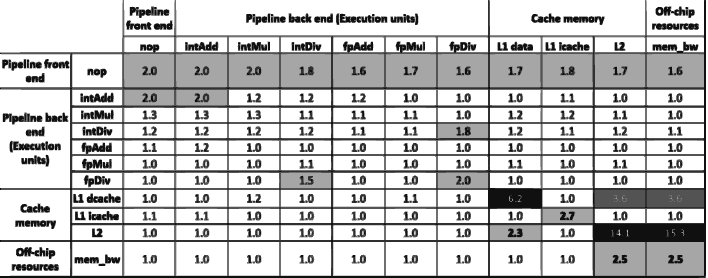
\includegraphics[width=\textwidth]{\chapterdirectory/figure/micro_bench/atom_stress.pdf}
\end{center}
\caption{Slowdown factor on the Intel Atom Z530 (taken from \cite{10.1145/2086696.2086713})}%
\label{fig:micro_bench:atom_stress}
\end{figure}

Figure~\ref{fig:micro_bench:atom_stress} shows the approach of
\cite{10.1145/2086696.2086713} working at its best. This is the result on an
Intel Atom Z530, which features a single core capable of running two parallel
threads. The lines correspond to the benchmark being measured, the columns
correspond to the target of the benchmark being used as a source of
interference.

\begin{figure}[hbt!]
\begin{center}
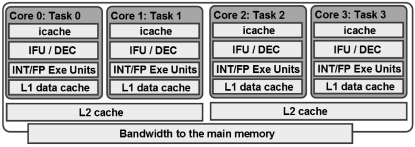
\includegraphics[width=0.6\textwidth]{\chapterdirectory/figure/micro_bench/core2quad.png}
\end{center}
\caption{The Intel Core2Quad architecture (taken
from \cite{10.1145/2086696.2086713})}%
\label{fig:micro_bench:core2quad}
\end{figure}

\begin{figure}[hbt!]
\begin{center}
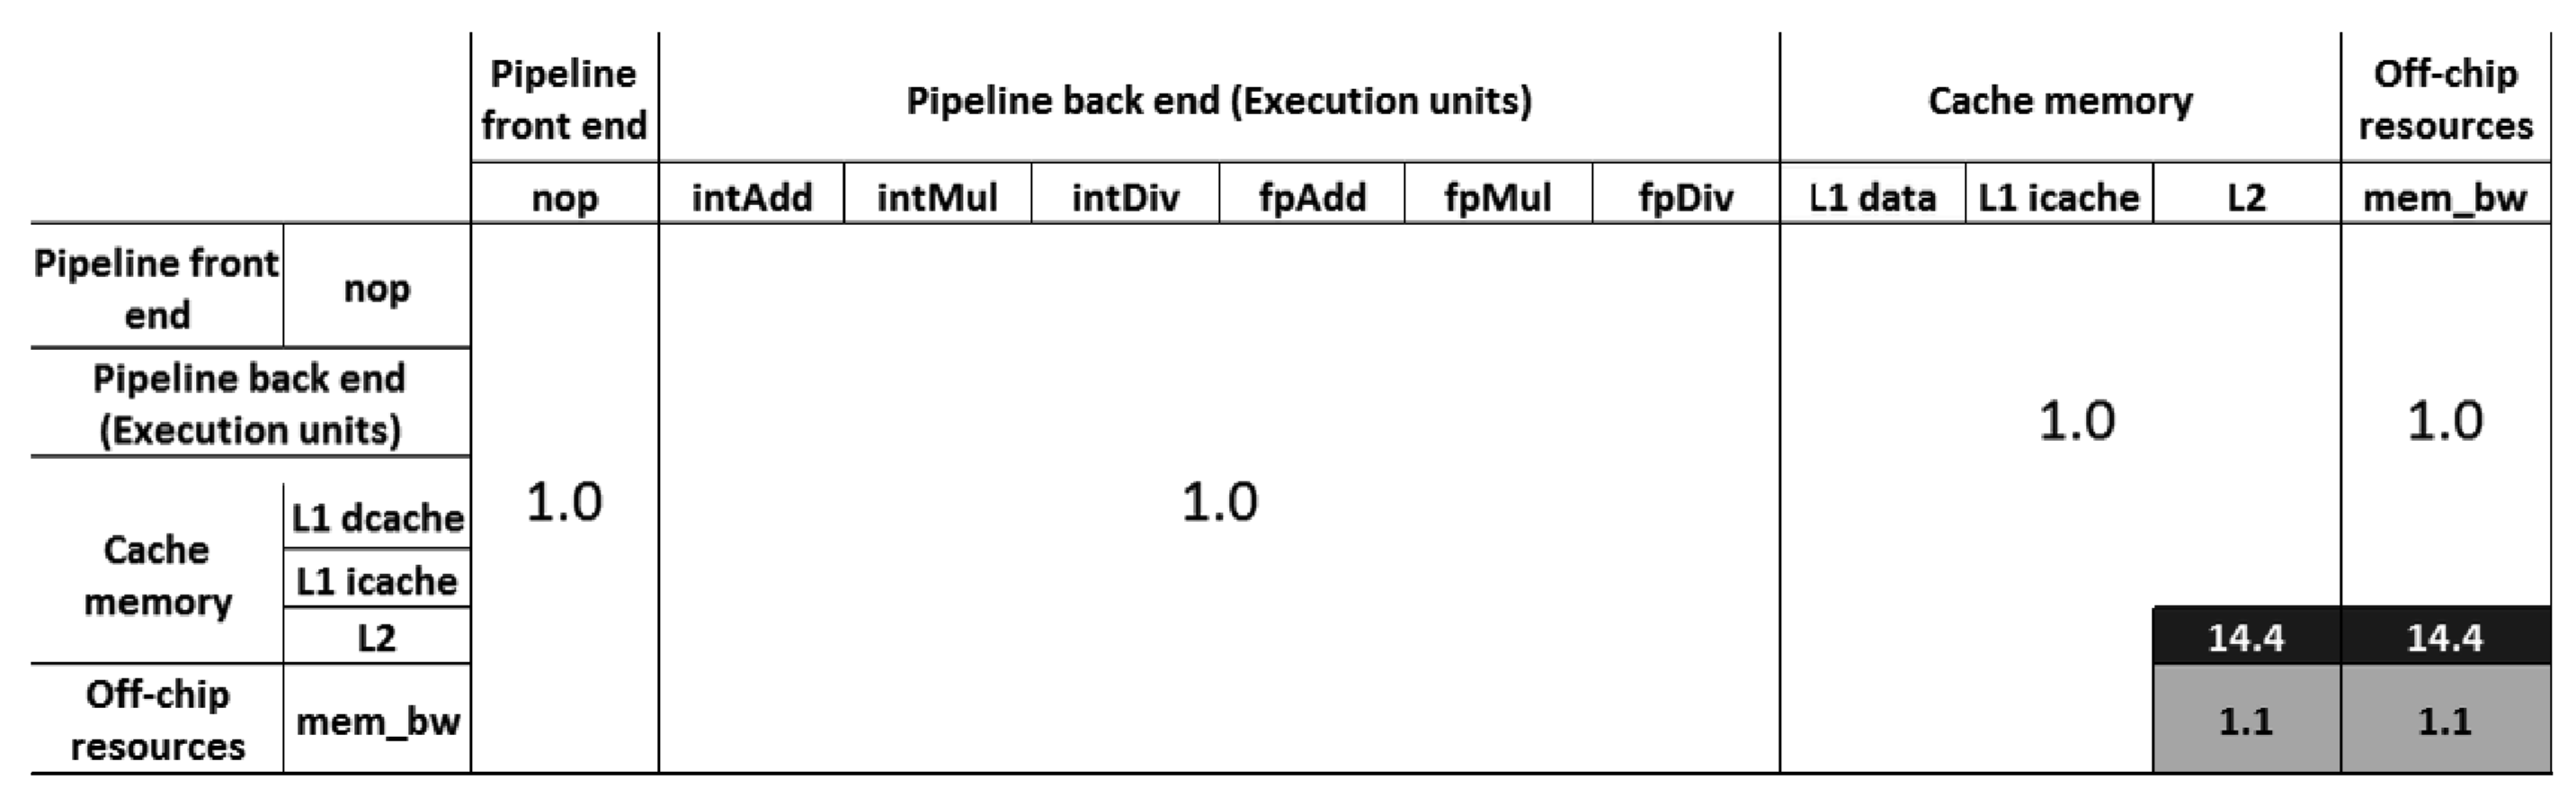
\includegraphics[width=\textwidth]{\chapterdirectory/figure/micro_bench/shared_cache_interference_detect.png}
\end{center}
\caption{Slowdown factor on the Intel Core2Quad within the same cluster (taken
from \cite{10.1145/2086696.2086713})}%
\label{fig:micro_bench:core2quad_stress}
\end{figure}

The application on a multi-core processor, however, is not as informative:
Figure~\ref{fig:micro_bench:core2quad_stress} shows the same experiment
performed within a cluster of an Intel Core2Quad (two separate cores that share
the same L2 cache, see Figure~\ref{fig:micro_bench:core2quad}). The results
indicate no unexpected slowdowns from the simultaneous use of components.
Information on slowdown due to simultaneous use of caches points is still
relevant and points to running two parallel cache intensive programs being
slower than one after the other.

\begin{figure}[hbt!]
\begin{center}
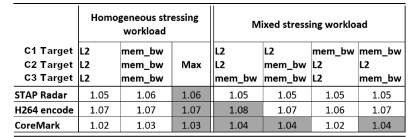
\includegraphics[width=0.5\textwidth]{\chapterdirectory/figure/micro_bench/simultaneous_stressing.png}
\end{center}
\caption{Standard benchmark interference on the Intel Core2Quad (taken
from \cite{10.1145/2086696.2086713})}%
\label{fig:micro_bench:core2quad_max_interference}
\end{figure}

\cite{10.1145/2086696.2086713} does not provide the analysis of potential
interference channels with more than two components in use simultaneously, but
it does analyze the slowdown factor suffered by some standard benchmark
applications running on one core when other components are being stressed by all
the other core.
The results are shown in
Figure~\ref{fig:micro_bench:core2quad_max_interference}. The observed slowdown
factors are very small, regardless of the components being stressed by the other
cores. This points to the use of standard benchmarks being poor indicators of
the worst slowdown that can be suffered because of interference. Indeed, none of
these results reflect the high slowdown factor that was obtained when even just
two cores stressed the same L2 cache. Thus, the effects of interference on an
application that uses the L2 cache more than those standard benchmarks is likely
to be much higher than what the results from
Figure~\ref{fig:micro_bench:core2quad_max_interference} would lead to believe.

\iffalse % Let's ignore the paper's actual contribution, shall we?
Figure~\ref{fig:micro_bench:atom_stress} shows the slowdown factors obtained by
this strategy on a Intel Atom Z530, which features a single core capable of
running two parallel threads. The lines correspond to the benchmark being
measured, the columns correspond to the target of the benchmark being used as
a source of interference.

The paper presents the same table for two other architectures: an Intel Pentium
D, with two cores each capable of a single thread; and an Intel Core2Quad
Q9550, with four cores, also only capable of a single thread. The resulting
slowdown factors for this particular set of shared resources for these two
architectures is considerably less impressive however, as only at most
two of these resources are actually shared by the separate cores (\textit{L2
cache}, and main memory access - \textit{mem\_bw}). Nevertheless, performing
such measurements does confirm that the resources are indeed not shared and
thus unable to interfere with one another, and the results do point out
L2 cache accesses to be a bottleneck on the Core2Quad architecture, with a
slowdown factor of $14.4$.

The results shown in \cite{10.1145/2086696.2086713}, especially those in
Figure~\ref{fig:micro_bench:atom_stress}, do make a strong argument against the
use of simultaneous multi-threading on a single core in applications with
real-time constraints, as having to taking into account the slowdown factor of
each of these shared resources makes the estimation of a precise worst-case
execution time that much more difficult. Unsurprisingly, such results are the
reason for simultaneous multi-threading being forbidden in aeronautical
contexts.
\fi

To summarize, the strategy employed here forms the basis of covert interference
channel identification, as it exposes potentially unknown links between
components, but it also provides some quantification of the architecture's
capabilities through the slowdown factor, and argues for the use of
micro-stressing benchmarks over that of standard ones for a true observation of
the maximum impact of interference, including for interference related to the
use of caches.

The next paper expands on this approach, by using performance monitors to
measure more than cycle counts, and thus learn more about how components
interact.

\stopallthesefloats
